\documentclass[plain]{pset}
\usepackage{dylanhu}

\title{Practice Midterm 2}
\author{Dylan Hu}
\prof{Professor Zhuolun Yang}
\course{APMA 0360 --- Partial Differential Equations}
\date{April 9, 2024}

\begin{document}

\maketitle

\pagebreak

\begin{problem}
Compute the Fourier sine series of \(x^2 + 1\) on \([0, \pi]\).
\end{problem}

\begin{solution}
    \begin{align*}
        a_n & = \frac{2}{\pi} \int_0^\pi (x^2 + 1) \sin(nx) \dd x                                                                                                                              \\
            & = \frac{2}{\pi} \int_0^\pi (x^2 + 1) \pdv{}{x} \left(-\frac{\cos(nx)}{n}\right) \dd x                                                                                            \\
            & = \frac{2}{\pi} \left[\left. (x^2 + 1) \left(-\frac{\cos(nx)}{n}\right) \right|_0^\pi - \int_0^\pi \left(-\frac{\cos(nx)}{n}\right) \pdv{}{x} (x^2 + 1) \dd x\right]             \\
            & = \frac{2}{\pi} \left[(\pi^2 + 1)\left(-\frac{\cos(n\pi)}{n}\right) - \left(-\frac{\cos(0)}{n}\right)\right] - \frac{2}{\pi}\int_0^\pi \left(-\frac{\cos(nx)}{n}\right) 2x \dd x \\
            & = \frac{2}{n\pi}\left(1-(\pi^2 + 1)(-1)^n\right) + \frac{4}{n\pi} \int_0^\pi x\cos(nx) \dd x                                                                                     \\
            & = \frac{2}{n\pi}\left(1-(\pi^2 + 1)(-1)^n\right) + \frac{4}{n\pi} \left[\left. x \left(\frac{\sin(nx)}{n}\right)\right|_0^\pi - \int_0^\pi \frac{\sin(nx)}{n} \dd x\right]       \\
            & = \frac{2}{n\pi}\left(1-(\pi^2 + 1)(-1)^n\right) - \frac{4}{n^2\pi} \int_0^\pi \sin(nx) \dd x                                                                                    \\
            & = \frac{2}{n\pi}\left(1-(\pi^2 + 1)(-1)^n\right) - \frac{4}{n^2\pi} \left[\left. -\frac{\cos(nx)}{n}\right|_0^\pi\right]                                                         \\
            & = \frac{2}{n\pi}\left(1-(\pi^2 + 1)(-1)^n\right) - \frac{4}{n^2\pi} \left(-\frac{(-1)^n - 1}{n}\right)                                                                           \\
            & = \frac{2}{n\pi}\left(1-(\pi^2 + 1)(-1)^n\right) - \frac{4}{n^3\pi}(1 - (-1)^n)                                                                                                  \\
    \end{align*}
    The Fourier sine series of \(x^2 + 1\) on \([0, \pi]\) is then
    \[\sum_{n=1}^\infty a_n \sin(nx).\]

    We can check that the Fourier series approximates \(x^2 + 1\) in \([0, \pi]\):
    \begin{figure}[h!]
        \centering
        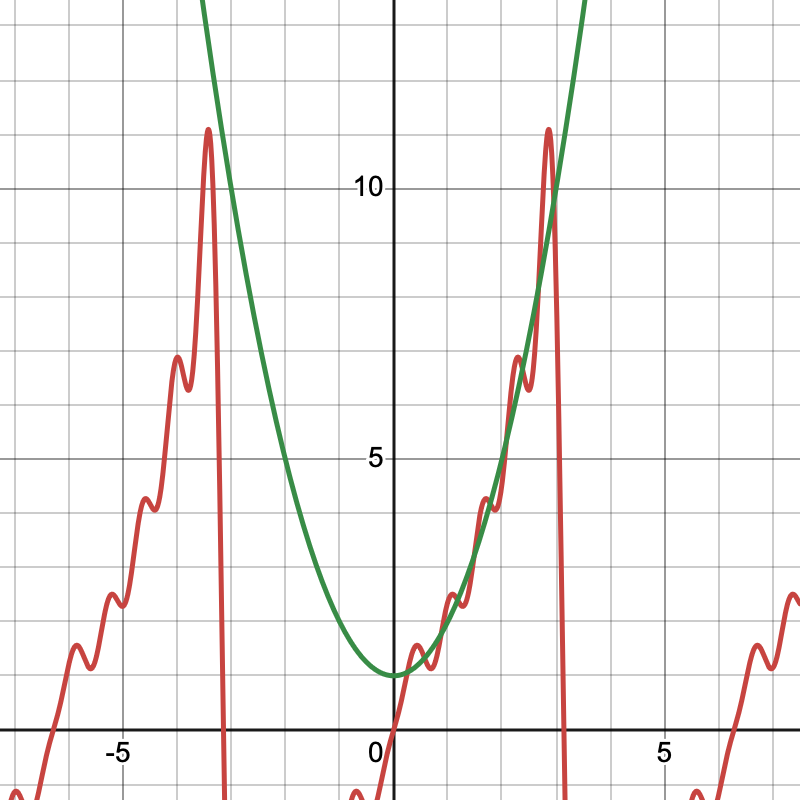
\includegraphics[width=0.35\textwidth]{1.png}
        \caption{\href{https://www.desmos.com/calculator/a7wlsqmh2f}{\texttt{https://www.desmos.com/calculator/a7wlsqmh2f}}}
    \end{figure}
\end{solution}

\pagebreak

\begin{problem}
Compute the Fourier sine series of \(\cos(x)\) on \([0, \pi]\). Does it converge to \(\cos(x)\) pointwise on \([0, \pi]\)? If not, at which points does it not converge?
\end{problem}

\begin{solution}
    \begin{align*}
        a_n & = \frac{2}{\pi} \int_0^\pi \cos(x) \sin(nx) \dd x                                                                                                                                 \\
            & = \frac{2}{\pi} \int_0^\pi \cos(x) \pdv{}{x} \left(-\frac{\cos(nx)}{n}\right) \dd x                                                                                               \\
            & = \frac{2}{\pi} \left[\left. \cos(x) \left(-\frac{\cos(nx)}{n}\right) \right|_0^\pi - \int_0^\pi \left(-\frac{\cos(nx)}{n}\right) \pdv{}{x} \cos(x) \dd x\right]                  \\
            & = \frac{2}{n\pi} \bigl(-\cos(\pi)\cos(n\pi) + \cos(0)\cos(0)\bigr) - \frac{2}{n\pi} \int_0^\pi \cos(nx) \sin(x) \dd x                                                             \\
            & = \frac{2}{n\pi} \left((-1)^n + 1\right) - \frac{2}{n\pi} \int_0^\pi \sin(x) \pdv{}{x} \left(\frac{\sin(nx)}{n}\right) \dd x                                                      \\
            & = \frac{2}{n\pi} \left((-1)^n + 1\right) - \frac{2}{n\pi} \left[\left. \sin(x) \left(\frac{\sin(nx)}{n}\right) \right|_0^\pi - \int_0^\pi \frac{\sin(nx)}{n} \cos(x) \dd x\right] \\
            & = \frac{2}{n\pi} \left((-1)^n + 1\right) + \frac{2}{n^2\pi} \int_0^\pi \cos(x) \sin(nx) \dd x                                                                                     \\
            & = \frac{2}{n\pi} \left((-1)^n + 1\right) + \frac{1}{n^2} a_n
    \end{align*}
    \[n^2 a_n = \frac{2n}{\pi} \left((-1)^n + 1\right) + a_n\]
    \[(n^2 - 1) a_n = \frac{2n}{\pi} \left((-1)^n + 1\right)\]
    \[a_n = \frac{2n\left((-1)^n + 1\right)}{\pi(n^2 - 1)}\]

    We can handle the special case of \(n = 1\) separately:
    \[a_1 = \frac{2}{\pi} \int_0^\pi \cos(x) \sin(x) \dd x\]
    We can use the fact that \(\sin(x)\) and \(\cos(x)\) are orthogonal, so \(\langle\cos(x), \sin(x)\rangle = \int \cos(x) \sin(x) \dd x = 0\). Therefore, \(a_1 = 0\).

    The Fourier sine series of \(\cos(x)\) on \([0, \pi]\) is then
    \[\sum_{n=2}^\infty a_n \sin(nx)\]
    where
    \[a_n = \frac{2n\left((-1)^n + 1\right)}{\pi(n^2 - 1)}.\]

    We can determine the pointwise convergence of the Fourier series by only checking the convergence of the series at the endpoints of the interval, as \(\cos(x)\) is continuous everywhere:
    \[\lim_{n \to \infty} \cos(0) = 1 \neq 0 = \lim_{n \to \infty} \sum_{n=2}^\infty a_n \sin(nx)\]
    \[\lim_{n \to \infty} \cos(\pi) = -1 \neq 0 = \lim_{n \to \infty} \sum_{n=2}^\infty a_n \sin(nx)\]
    Therefore, the Fourier series does not converge to \(\cos(x)\) pointwise on \([0, \pi]\), as it does not converge at \(x = 0\) and \(x = \pi\).
\end{solution}

\pagebreak

\begin{problem}
Solve
\[
    \begin{cases}
        \begin{aligned}
            u_t       & = tu_{xx}, &  & 0 < x < \pi, & t > 0, \\
            u(0, t)   & = 0,       &  & t > 0,       &        \\
            u(\pi, t) & = 0,       &  & t > 0,       &        \\
            u(x, 0)   & = x,       &  & 0 < x < \pi
        \end{aligned}
    \end{cases}
\]
using separation of variables.
\end{problem}

\begin{solution}
    Let \(u(x, t) = X(x)T(t)\). Then
    \[u_t = tu_{xx} \implies X(x)T'(t) = tX''(x)T(t) \implies \frac{X''(x)}{X(x)} = \frac{1}{t}\frac{T'(t)}{T(t)} = \lambda\]

    We recall that a solution for the homogeneous Dirichlet boundary conditions is
    \[X(x) = c \sin(nx)\]
    for a constant \(c\), \(n = 1, 2, 3, \ldots\), and \(\lambda = -n^2\). We can then solve the ODE in \(T(t)\):

    \[\frac{1}{t}\frac{T'(t)}{T(t)} = -n^2\]
    \[\frac{T'(t)}{T(t)} = -n^2t\]
    \[\dv{}{t} \ln T(t) = -n^2t\]
    \[\ln T(t) = -\frac{n^2}{2}t^2 + c\]
    \[T(t) = e^{-\frac{n^2}{2}t^2 + c} = Ce^{-\frac{n^2}{2}t^2}\]

    The general solution is then
    \[u(x, t) = \sum_{n=1}^\infty a_n e^{-\frac{n^2}{2}t^2}\sin(nx)\]

    We can determine the coefficients \(a_n\) by using the initial condition:
    \[u(x, 0) = \sum_{n=1}^\infty a_n \sin(nx) = x\]
    Recall from lecture that the Fourier sine series of \(x\) on \([0, \pi]\) is
    \[x \stackrel{L^2}{=} \sum_{n=1}^\infty a_n \sin(nx)\]
    where
    \[a_n = (-1)^{n+1} \frac{2}{n}.\]

    Therefore, the solution to the PDE is
    \[u(x, t) = \sum_{n=1}^\infty (-1)^{n+1} \frac{2}{n} e^{-\frac{n^2}{2}t^2}\sin(nx).\]
\end{solution}

\pagebreak

\begin{problem}
Solve
\[
    \begin{cases}
        \begin{aligned}
            u_{tt}    & = 4u_{xx},             &  & 0 < x < \pi, & t > 0, \\
            u(0, t)   & = 0,                   &  & t > 0,       &        \\
            u(\pi, t) & = 0,                   &  & t > 0,       &        \\
            u(x, 0)   & = x,                   &  & 0 < x < \pi, &        \\
            u_t(x, 0) & = \sin(4x) + 5\sin(5x) &  & 0 < x < \pi
        \end{aligned}
    \end{cases}
\]
using separation of variables.
\end{problem}

\begin{solution}
    Let \(u(x, t) = X(x)T(t)\). Then
    \[u_{tt} = 4u_{xx} \implies X(x)T''(t) = 4X''(x)T(t) \implies \frac{X''(x)}{X(x)} = \frac{1}{4}\frac{T''(t)}{T(t)} = \lambda\]

    We recall that a solution for the homogeneous Dirichlet boundary conditions is
    \[X(x) = c \sin(nx)\]
    for a constant \(c\), \(n = 1, 2, 3, \ldots\), and \(\lambda = -n^2\). We can then solve the ODE in \(T(t)\):
    \[\frac{1}{4}\frac{T''(t)}{T(t)} = -n^2\]
    \[T''(t) = -4n^2T(t)\]
    We recall that the general solution to this ODE is
    \[T(t) = c_1\cos(2nt) + c_2\sin(2nt)\]

    The general solution is then
    \[u(x, t) = \sum_{n=1}^\infty \bigl(a_n\cos(2nt) + b_n\sin(2nt)\bigr)\sin(nx)\]

    We can determine the coefficients \(a_n\) and \(b_n\) by using the initial conditions:
    \[u(x, 0) = \sum_{n=1}^\infty a_n \sin(nx) = x\]

    Recall from lecture that the Fourier sine series of \(x\) on \([0, \pi]\) is
    \[x \stackrel{L^2}{=} \sum_{n=1}^\infty a_n \sin(nx)\]
    where
    \[a_n = (-1)^{n+1} \frac{2}{n}.\]

    Turning to the second initial condition:
    \[u_t(x, t) = \sum_{n=1}^\infty 2n\bigl(-a_n\sin(2nt) + b_n\cos(2nt)\bigr)\sin(nx)\]
    \[u_t(x, 0) = \sum_{n=1}^\infty 2n b_n \sin(nx) = \sin(4x) + 5\sin(5x)\]

    Comparing terms, we see that \(b_4 = \frac{1}{8}\), \(b_5 = \frac{1}{2}\), and \(b_k = 0\) for \(k \neq 4, 5\).

    Therefore, the solution to the PDE is
    \[u(x, t) = \frac{1}{8}\sin(8t)\sin(4x) + \frac{1}{2}\sin(10t)\sin(5x) + \sum_{n=1}^\infty (-1)^{n+1} \frac{2}{n}\cos(2nt)\sin(nx).\]
\end{solution}

\pagebreak

\begin{problem}
Use the energy method to show that the only solution to the heat-like equation with periodic boundary conditions
\[
    \begin{cases}
        \begin{aligned}
            u_t       & = 4u_{xx} - 3u, &  & 0 < x < \pi, & t > 0, \\
            u(0, t)   & = u(\pi, t),    &  & t > 0,       &        \\
            u_x(0, t) & = u_x(\pi, t),  &  & t > 0,       &        \\
            u(x, 0)   & = 0,            &  & 0 < x < \pi
        \end{aligned}
    \end{cases}
\]
is zero.
\end{problem}

\begin{solution}
    We can multiply the PDE by \(u\) and integrate over \([0, \pi]\):
    \[\int_0^\pi u_t u \dd x = \int_0^\pi (4u_{xx} - 3u)u \dd x\]
    \[\int_0^\pi \pdv{}{t}\left(\frac{1}{2}u^2\right) \dd x = \int_0^\pi 4u_{xx}u \dd x - 3\int_0^\pi u^2 \dd x\]
    \[\dv{}{t} \int_0^\pi \frac{1}{2}u^2 \dd x = \int_0^\pi 4u_{xx}u \dd x - 3\int_0^\pi u^2 \dd x\]
    Let \(E(t) = \int_0^\pi \frac{1}{2}u^2 \dd x \geq 0\). Then
    \begin{align*}
        \dv{E}{t} & = 4\int_0^\pi u_{xx}u \dd x - 3\int_0^\pi u^2 \dd x                                                       \\
                  & = 4\left.u_x u\right|_0^\pi - 4\int_0^\pi u_x^2 \dd x - 3\int_0^\pi u^2 \dd x                             \\
                  & = 4\left[u_x(\pi, t)u(\pi, t) - u_x(0, t)u(0, t)\right] - 4\int_0^\pi u_x^2 \dd x - 3\int_0^\pi u^2 \dd x \\
                  & = 0 - 4\int_0^\pi u_x^2 \dd x - 3\int_0^\pi u^2 \dd x                                                     \\
                  & \leq 0
    \end{align*}
    Then \(0 \leq E(t) \leq E(0) = 0\), so \(E(t) = 0\). Therefore, \(u(x, t) = 0\).
\end{solution}

\pagebreak

\begin{problem}
Consider the system of equations
\[
    \begin{cases}
        \begin{aligned}
            u_t & = 4u_{xx} - 3u_x - 5uv^2, \\
            v_t & = -3uv^2.
        \end{aligned}
    \end{cases}
\]
Find a system of ODEs for \(U\) and \(V\), where \(U, V\) are the traveling wave profiles \(u(x, t) = U(z), \ v(x, t) = V(z), \ z = x - ct\).
\end{problem}

\begin{solution}
    We have the following system:
    \[
        \begin{cases}
            \begin{aligned}
                u(x, t) & = U(x - ct) & = U(z), \\
                v(x, t) & = V(x - ct) & = V(z).
            \end{aligned}
        \end{cases}
        \implies
        \begin{cases}
            \begin{aligned}
                u_t    & = \dv{U}{z}\dv{z}{t}  &  & = -cU'(z), \\
                v_t    & = \dv{V}{z}\dv{z}{t}  &  & = -cV'(z), \\
                u_x    & = \dv{U}{z}\dv{z}{x}  &  & = U'(z),   \\
                u_{xx} & = \dv{U'}{z}\dv{z}{x} &  & = U''(z).
            \end{aligned}
        \end{cases}
    \]
    Now we can substitute these into the original system:
    \[
        \begin{cases}
            \begin{aligned}
                -cU'(z) & = 4U''(z) - 3U'(z) - 5UV^2, \\
                -cV'(z) & = -3UV^2.
            \end{aligned}
        \end{cases}
    \]
\end{solution}

\pagebreak

\begin{problem}
Use separation of variables to solve
\[
    \begin{cases}
        \begin{aligned}
            u_{xx} + u_{yy} & = 0,        &  & 0 < x, y < \pi, \\
            u(x, 0)         & = 0,        &  & 0 < x < \pi,    \\
            u(x, \pi)       & = 0,        &  & 0 < x < \pi,    \\
            u_x(0, y)       & = \sin(2y), &  & 0 < y < \pi,    \\
            u_x(\pi, y)     & = 0,        &  & 0 < y < \pi,    \\
        \end{aligned}
    \end{cases}
\]
\textbf{Note:} \((\cosh(x))' = \sinh(x)\), \((\sinh(x))' = \cosh(x)\). No negative signs for the derivatives of hyperbolic sine/cosine functions.
\end{problem}

\begin{solution}
    Let \(u(x, y) = X(x)Y(y)\). Then
    \[u_{xx} + u_{yy} = 0 \implies X''Y + XY'' = 0 \implies -\frac{X''}{X} = \frac{Y''}{Y} = \lambda\]

    We first solve the ODE in \(Y(y)\):
    \[
        \begin{cases}
            \begin{aligned}
                Y''(y) & = \lambda Y(y), \\
                Y(0)   & = 0,            \\
                Y(\pi) & = 0.
            \end{aligned}
        \end{cases}
    \]
    Recall that a solution to the homogeneous Dirichlet boundary conditions is
    \[Y(y) = c \sin(ny)\]
    for a constant \(c\), \(n = 1, 2, 3, \ldots\), and \(\lambda = -n^2\). We can then solve the ODE in \(X(x)\):
    \[X''(x) = -\lambda X(x) = n^2 X(x)\]
    Recall the general solution
    \[X(x) = Ae^{nx} + Be^{-nx}\]
    which can be rewritten using the hyperbolic sine and cosine functions as
    \[X(x) = \tilde{A}\sinh(nx) + \tilde{B}\cosh(nx).\]

    The solution with the homogeneous Dirichlet boundary conditions is then
    \[u(x, y) = \sum_{n=1}^\infty \bigl(a_n\sinh(nx) + b_n\cosh(nx)\bigr)\sin(ny).\]

    We now determine the coefficients \(a_n\) and \(b_n\) with the other boundary conditions.

    First, we compute the partial derivative of \(u\) with respect to \(x\):
    \[u_x(x, y) = \sum_{n=1}^\infty n\bigl(a_n\cosh(nx) + b_n\sinh(nx)\bigr)\sin(ny)\]

    With the \(u_x(0, y) = \sin(2y)\) boundary condition:
    \[u_x(0, y) = \sum_{n=1}^\infty n a_n \sin(ny) = \sin(2y)\]
    Comparing terms, we see that \(a_2 = \frac{1}{2}\) and \(a_k = 0\) for \(k \neq 2\).

    With the \(u_x(\pi, y) = 0\) boundary condition:
    \[u_x(\pi, y) = \sum_{n=1}^\infty n\bigl(a_n\cosh(n\pi) + b_n\sinh(n\pi)\bigr)\sin(ny) = 0\]
    We know that the \(n\) factor is strictly positive, and we would like to assume \(\sin(ny) \neq 0\) for all \(n\) in order to avoid trivial solutions. Therefore, we must have
    \[\sum_{n=1}^\infty a_n\cosh(n\pi) + b_n\sinh(n\pi) = 0\]
    We know that \(a_k = 0\) for \(k \neq 2\), so we have
    \[\frac{1}{2}\cosh(2\pi) + \sum_{n=1}^\infty b_n\sinh(n\pi) = 0\]

    We can choose \(b_k = 0\) for all \(k \neq 2\):
    \[\frac{1}{2}\cosh(2\pi) + b_2\sinh(2\pi) = 0\]

    Then \(b_2 = -\frac{\cosh(2\pi)}{2\sinh(2\pi)}\), and a solution to the PDE is
    \[u(x, y) = \frac{1}{2}\sinh(2x)\sin(2y) - \frac{\cosh(2\pi)}{2\sinh(2\pi)}\cosh(2x)\sin(2y).\]
\end{solution}

\end{document}
